The search for the exotic decay of the 125\GeV Higgs boson to two light neutral scalars decaying to a pair of bottom quarks and a pair of tau leptons ($h \rightarrow aa \rightarrow bb\tau\tau$) is based on proton-proton collision data at a center-of-mass energy 13 TeV collected in Run-2 of data-taking, spanning the data-taking years 2016, 2017, and 2018. The datasets used and the triggers used to collect the data are described in Section \ref{section:data-datasets}. Section \ref{section:mc-samples} describes the Monte Carlo simulated samples that are used to model the $h \rightarrow aa \rightarrow bb\tau\tau$ signal and background Standard Model processes. Lastly, in order to obtain a better description of Standard Model backgrounds that contain two tau leptons, a data-Monte Carlo hybrid technique is used to generate embedded samples which model processes with genuine $\tau\tau$ in the final state, as detailed in Section \ref{section:embedded-samples}. All samples are listed in Appendix \ref{appendix-a:samples}.

\section{Datasets used}
\label{section:data-datasets}
The $h \rightarrow aa \rightarrow bb\tau\tau$ analysis~\cite{CMS-HIG-22-007} is based on proton-proton collision data at a center-of-mass energy of 13 TeV collected in full Run-2 (2016-18) with the CMS detector. The data analyzed corresponds to a total integrated luminosity of 138 fb$^{-1}$ (36.33 fb$^{-1}$ for 2016, 41.53 fb$^{-1}$ for 2017, and 59.74 fb$^{-1}$ for 2018)~\cite{CMS-LUM-17-001}~\cite{CMS-LUM-17-004}~\cite{CMS-LUM-18-002}. The cumulative delivered and recorded luminosity versus time for 2015-2018 is shown in Fig. \ref{fig:integrated-luminosity-Run-2}.

\begin{figure}[ht]
    \centering
    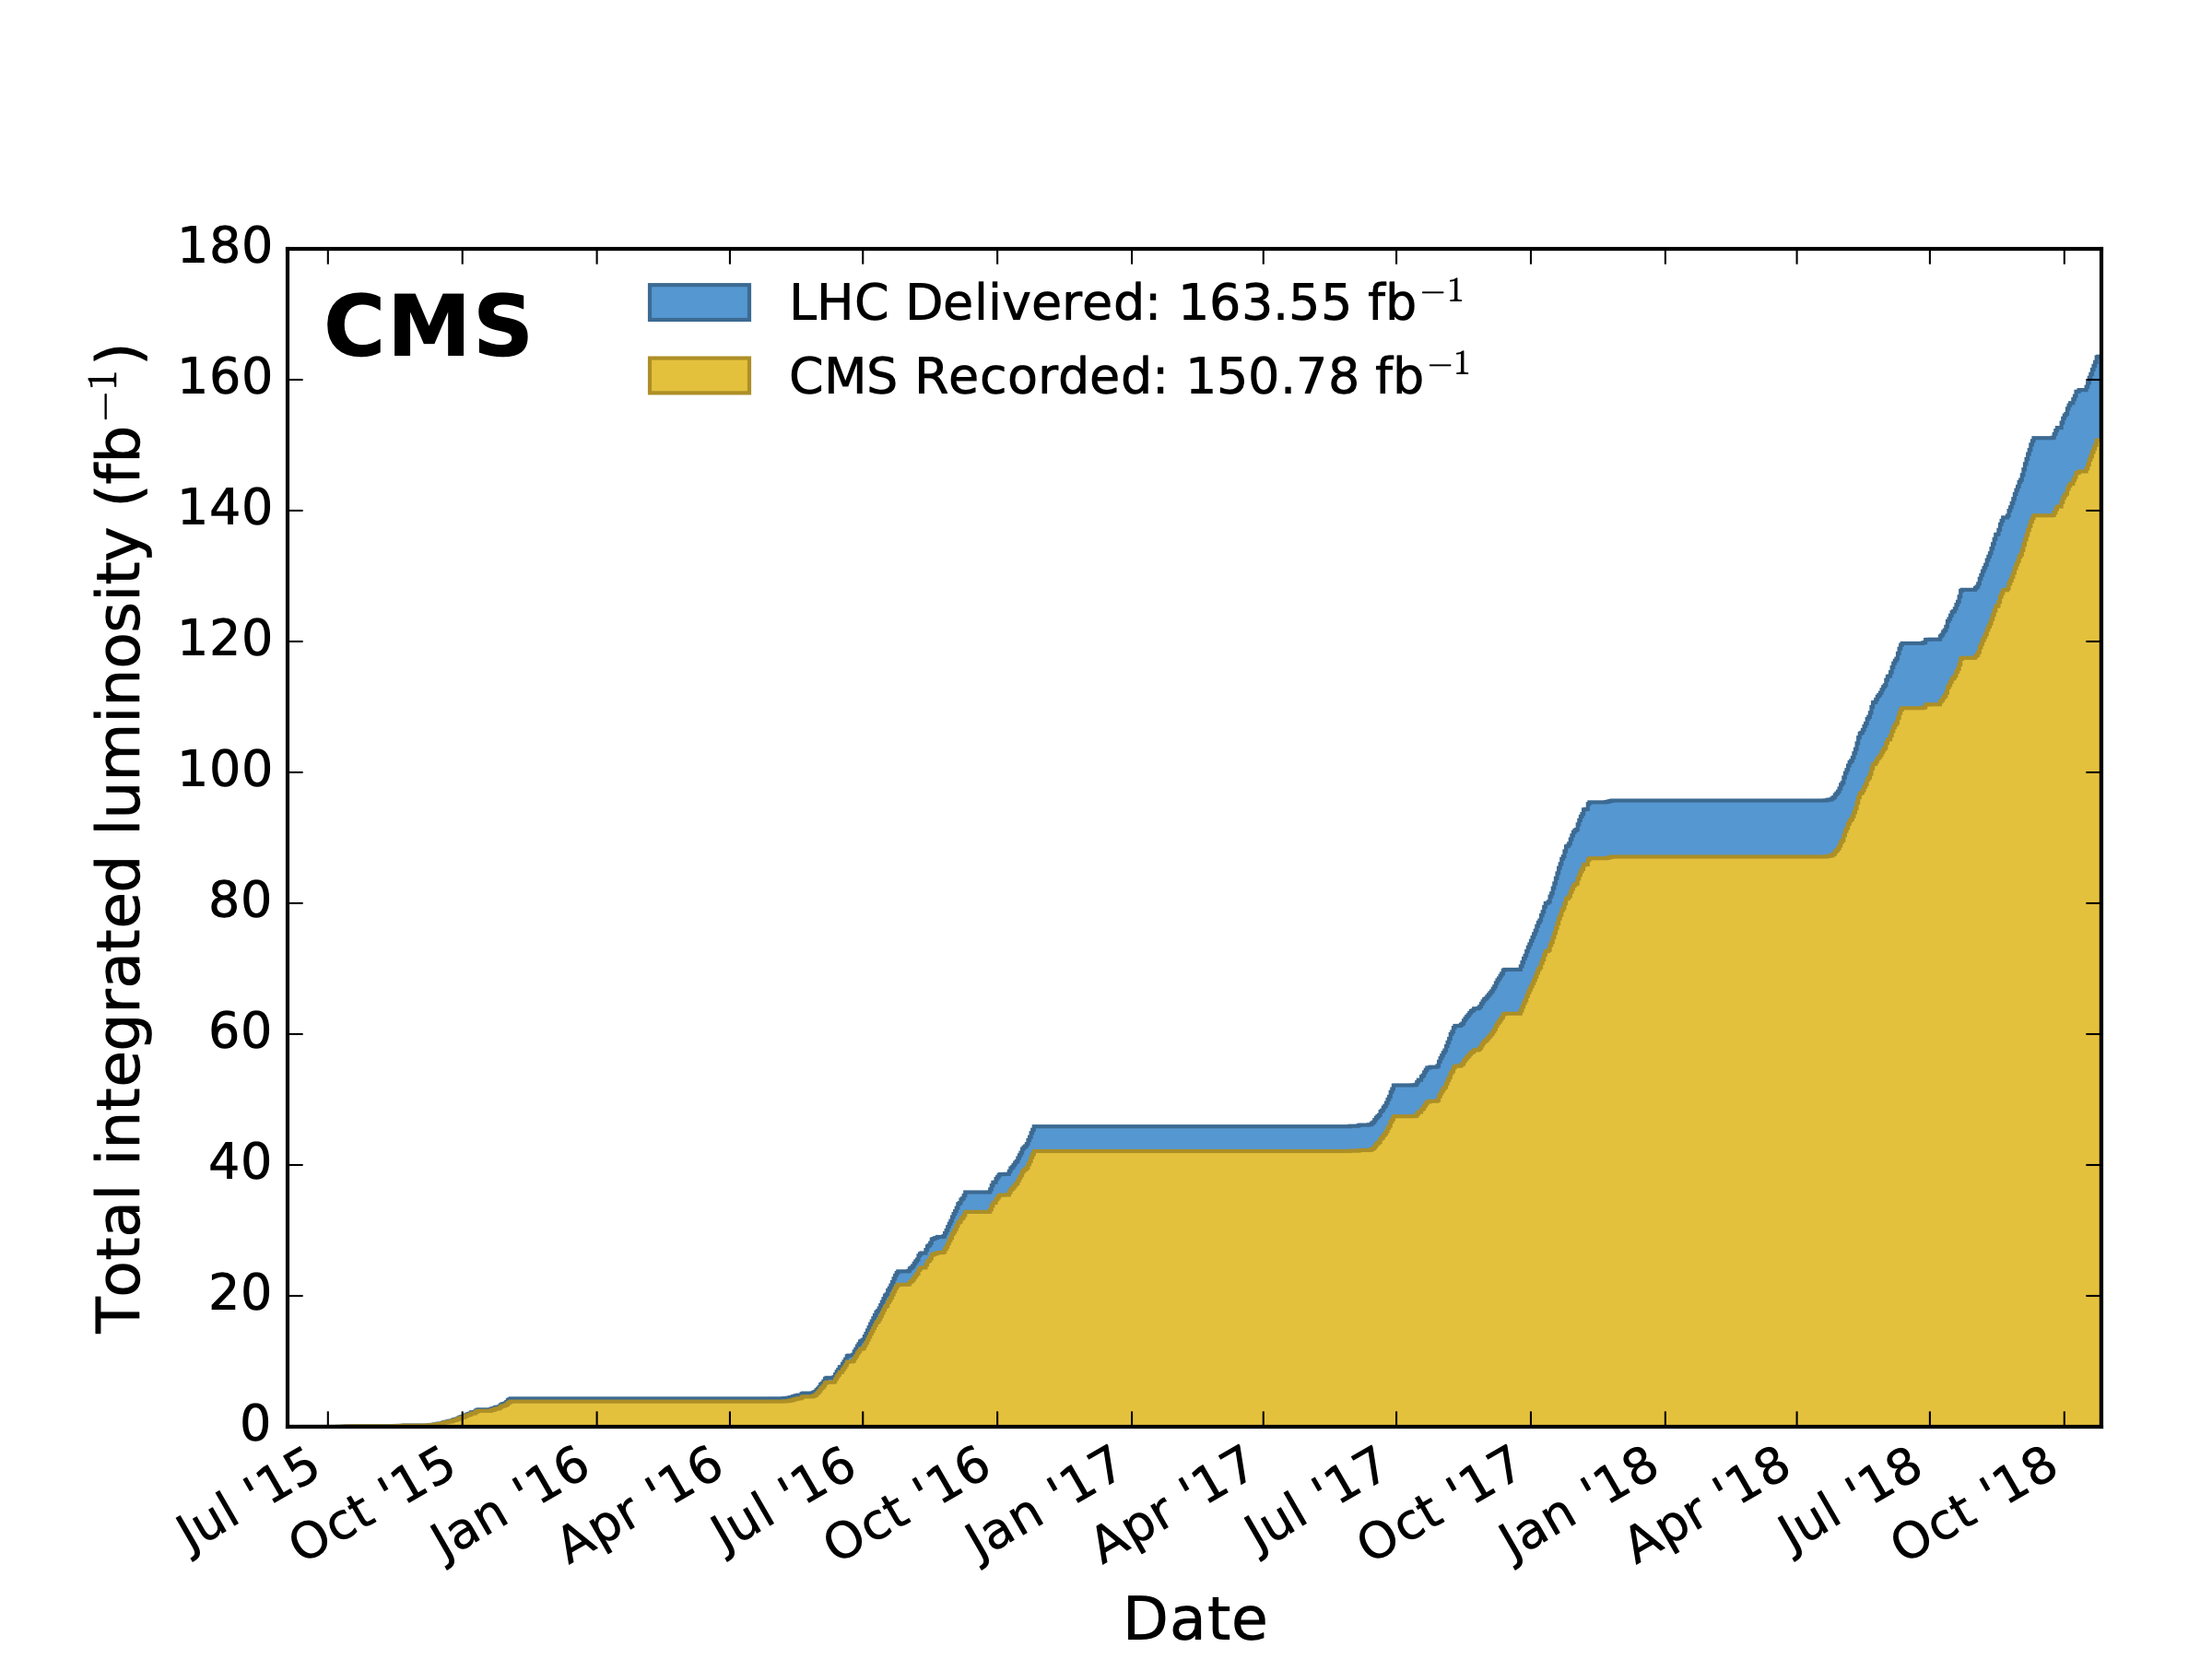
\includegraphics[width=10cm]{figures/ch-4-datasets-monte-carlo/int_lumi_allcumulative_pp_run2}
    \caption[Cumulative delivered and recorded luminosity versus time for 2015-2018 at CMS, in proton-proton collision data only, at nominal center-of-mass energy.]{Cumulative delivered and recorded luminosity versus time for 2015-2018 at CMS, in proton-proton collision data only, at nominal center-of-mass energy~\cite{twiki_Lumi_Public_Results}.} 
    \label{fig:integrated-luminosity-Run-2}
\end{figure}

Data collected with the single muon trigger is used for the $\mu\tau_{h}$ channel. For the $e\tau_{h}$ channel, data collected with the single electron trigger is used; and for the $e\mu$ channel, data collected with the electron $+$ muon trigger is used. A more in-depth discussion of the triggers used follows in a later section. The datasets are listed in Appendix \ref{appendix-a:samples} in Tables~\ref{tab:2016datasets}, \ref{tab:2017datasets}, and \ref{tab:2018datasets}.

\section{Monte Carlo samples}
\label{section:mc-samples}
Modeling and computing observables originating from arbitrary physics processes at the tree level and at next-to-leading order (NLO) is performed by Monte Carlo (MC) event generators, such as Powheg and MadGraph5\_amC\@NLO~\cite{Alwall_2014}~\cite{Frederix_2018}. The information generated, e.g. the computation of the differential cross sections and kinematics of the final state particles, is saved in a compressed file and used to generate MC samples that are used in physics analyses. The samples are digitized using GEANT4~\cite{agostinelli_geant4simulation_2003}, a platform used at the LHC and other facilities to comprehensively simulate the passage of particles through matter. The digitized samples are passed through the same detector reconstruction as real data events collected in the detector. The MC background samples used in this analysis for 2016-2018 are listed in Appendix \ref{appendix-a:samples} in Tables~\ref{tab:2016mcbkg}, \ref{tab:2017mcbkg}, and \ref{tab:2018mcbkg}.

The samples for modeling the signal ($h \rightarrow aa \rightarrow 2b2\tau$ and $h\rightarrow a_1 a_2$) in the 2HDM+S and TRSM are generated at tree-level, for a range of masses of the light neutral scalar $a$. For $h \rightarrow aa$, the mass hypotheses for the $a$ range from $m_a = (12 \,\text{GeV}, 62.5 \,\text{GeV})$. For $h \rightarrow a_1 a_2$, the mass hypotheses for the two light scalars span combinations of $m_{a1}$, $m_{a2}$ ranging from $(12 \,\text{GeV}, 62.5 \,\text{GeV})$ for the two scalars. The MC signal samples used in this analysis for 2016-2018 are listed in Appendix \ref{appendix-a:samples} in Tables~\ref{tab:2016signal}, \ref{tab:2017signal} and \ref{tab:2018signal}. 


\section{Embedded samples}
\label{section:embedded-samples}
An important background for Higgs boson studies and searches for additional Higgs bosons is the decay of $Z$ bosons into pairs of $\tau$ leptons ($Z \rightarrow \tau\tau$). An embedded technique was developed in the context of Standard Model Higgs to $\tau\tau$ measurements, to model $Z \rightarrow \tau\tau$ decays, and was expanded to also model all Standard Model processes that contain $\tau\tau$~\cite{CMS-TAU-18-001}. The embedded technique has since been used successfully at CMS for the Standard Model $H \rightarrow \tau\tau$ measurement, as well as searches for minimal supersymmetric extensions to the Standard Model (MSSM)~\cite{CMS-HIG-13-021}~\cite{CMS-HIG-19-010}. 

The advantage of the embedded technique is that aspects of the event that are difficult to model and describe are directly taken from data, resulting in a better data description than can be achieved with only the $Z \rightarrow \tau\tau$ simulation~\cite{CMS-TAU-18-001}. The simulation must be tuned extensively to accurately model aspects of the data, such as time-dependent pile-up profiles, the production of additional jets, e.g. in multijet and vector boson fusion topologies, the number of reconstructed primary interaction vertices, and the missing transverse momentum $p_{T}^{\text{miss}}$. Since all events with genuine $\tau\tau$ are estimated with samples made with the embedded technique (referred to as embedded samples from here on), events in Monte Carlo simulation with genuine $\tau\tau$ are not used, in order to avoid double-counting.

Fig. \ref{fig:embedded-schematic} shows a schematic of how embedded samples are produced. Data events containing $Z \rightarrow \mu\mu$ decays are selected. In these events, all energy deposits of the recorded muons are removed, and are replaced with simulated tau leptons with the same kinematic properties as the removed muons. This results in a hybrid data format containing information from both observed and simulated events, as illustrated in Fig. \ref{fig:embedded-schematic}~\cite{CMS-TAU-18-001}. The embedded samples used for the years 2016-2018 are listed in Appendix \ref{appendix-a:samples} in Tables~\ref{tab:2016emb}, \ref{tab:2017emb}, and \ref{tab:2018emb}.

\begin{figure}[ht]
    \centering
    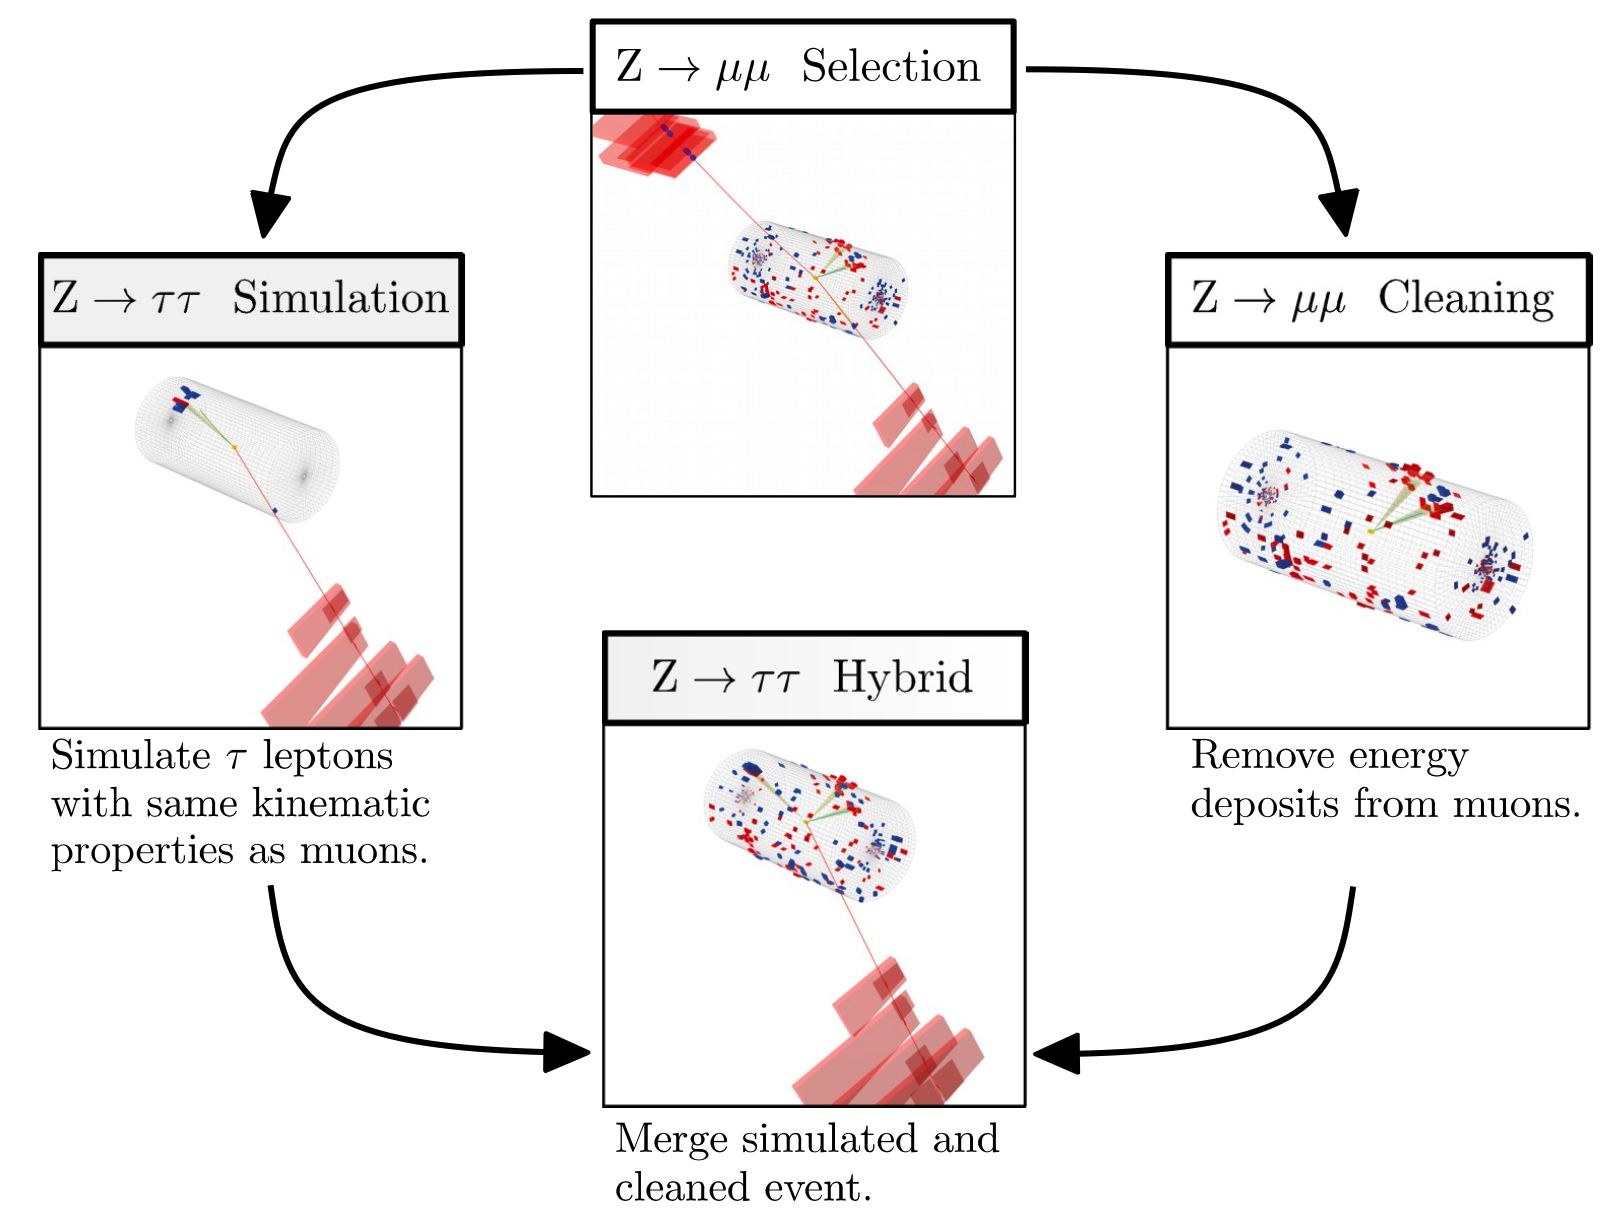
\includegraphics[width=13cm]{figures/ch-4-datasets-monte-carlo/embedded_schematic}
    \caption[Schematic view of the four main steps of the embedding technique for $\tau$ leptons.]{Schematic view of the four main steps of the embedding technique for $\tau$ leptons, as described in Section \ref{section:embedded-samples}~\cite{CMS-TAU-18-001}. A $Z \rightarrow \mu\mu$ event is selected in data (\textit{$Z\rightarrow \mu\mu$ selection}), all of the energy deposits associated with the muons are removed (\textit{$Z \rightarrow \mu\mu$ cleaning}), and two $\tau$ leptons and their decays are simulated in an empty detector (\textit{$Z \rightarrow \tau\tau$ simulation}). Lastly, all energy deposits of the simulated $\tau$ decays are combined with the data event (\textit{$Z \rightarrow \tau\tau$ hybrid}).} 
    \label{fig:embedded-schematic}
\end{figure}

In the selection step of the embedded technique, events are selected with at least one of a set of $\mu\mu$ trigger paths, which require $p_{T} > 17 (8)$ GeV for the leading (sub-leading) muons, and a minimum requirement between 3.8 and 8.0 GeV on the invariant di-muon mass $m_{\mu\mu}$~\cite{CMS-TAU-18-001}. The offline reconstructed muons must match the objects at trigger level and also have offline $p_{T} > 17 (8)$ GeV. They must have $|\eta| < 2.4$ and be located at a  distance $|d_z| < 0.2$ cm to the primary vertex along the beam axis. To form a Z boson candidate, each muon is required to originate from a global muon track. The muon pairs must have opposite charges with an invariant mass of $m_{\mu\mu} > 20$ GeV. If more than two di-muon pairs are found, the pair with the invariant mass closest to the Z boson mass (91.19 GeV) is chosen. 

This selection is designed to be tight enough to ensure a high purity of genuine $\mu\mu$ events, and also loose enough to minimize biases of the embedded event samples. Isolation requirements are avoided, since they would introduce a bias towards less hadronic activity in the vicinities of the embedded leptons that will appear more isolated than expected in data. The selection results in an expected mixture of events summarized in Table \ref{table:embedded_mixture_composition} from~\cite{CMS-TAU-18-001}. $Z \rightarrow \mu\mu$ is the dominant process modeled by the embedded technique, with $t\bar{t}$, QCD, and diboson and single top processes becoming more significant when considering events with b-tag jets.


\begin{table}[ht]
    \centering
    \begin{tabular}{|cccc|}
    \hline
    \multicolumn{4}{|c|}{Fraction (\%)}                                                                                                             \\ \hline
    \multicolumn{1}{|c|}{Process}                  & \multicolumn{1}{c|}{Inclusive} & \multicolumn{1}{c|}{$m_{\mu\mu} > 70$ GeV} & N(b-tag jets) $> 0$ \\ \hline
    \multicolumn{1}{|c|}{$Z \rightarrow \mu\mu$}   & \multicolumn{1}{c|}{97.36}     & \multicolumn{1}{c|}{99.11}                 & 69.25            \\
    \multicolumn{1}{|c|}{QCD}                      & \multicolumn{1}{c|}{0.84}      & \multicolumn{1}{c|}{0.10}                  & 2.08             \\
    \multicolumn{1}{|c|}{$t\bar{t}$}               & \multicolumn{1}{c|}{0.78}      & \multicolumn{1}{c|}{0.55}                  & 25.61            \\
    \multicolumn{1}{|c|}{$Z \rightarrow \tau\tau$} & \multicolumn{1}{c|}{0.71}      & \multicolumn{1}{c|}{0.05}                  & 0.57             \\
    \multicolumn{1}{|c|}{Diboson, single t}        & \multicolumn{1}{c|}{0.17}      & \multicolumn{1}{c|}{0.17}                  & 2.35             \\
    \multicolumn{1}{|c|}{W+jets}                   & \multicolumn{1}{c|}{0.08}      & \multicolumn{1}{c|}{0.02}                  & 0.14             \\ \hline
    \end{tabular}
    \caption[Expected event composition after selecting two muons in the embedded technique, before additional cuts (i.e. inclusive), and after adding a requirement on the di-muon mass $m_{\mu\mu} > 70$ GeV, or a requirement on the number of b-tag jets in the event.]{Expected event composition after selecting two muons in the embedded technique~\cite{CMS-TAU-18-001}, before additional cuts (i.e. inclusive, \textit{column 2}), and after adding a requirement on the di-muon mass $m_{\mu\mu} > 70$ GeV (\textit{column 3}), or a requirement on the number of b-tag jets in the event (\textit{column 4}).}
    \label{table:embedded_mixture_composition}
\end{table}
